\documentclass{article}
\usepackage[utf8]{inputenc}
\usepackage{amsmath}
\usepackage{booktabs}
\usepackage[margin=1in]{geometry}
\usepackage{setspace}
\usepackage{graphicx}

\title{\vspace{-2cm} Bayesian Hierarchical Model for Pitch Efficiency in Major League Baseball}
\author{Jacob Andros}
\date{December 9, 2021}

\linespread{1.08}
\begin{document}

\maketitle

\section{Introduction}

The threshold for removing a starting pitcher from a baseball game has been a highly contested topic in professional baseball for the past decade. As multi-inning relief pitchers become more common in the game, it is not uncommon to see the manager remove his starter after 80 pitches, whereas the norm used to be much higher (sometimes 120 or 130). In the MLB, the 2021 regular season only saw 691 instances where the starting pitcher threw at least 100 pitches; for comparison, the 2008 season had over 2000 such games. To put that in context, there are 2,430 games played in the MLB regular season with two starting pitchers in each, for a total of 4,680 starts. With starting pitchers being limited to fewer pitches than ever before, their utility is maximized if they can get through innings using fewer pitches. Pitches per inning (abbreviated as P/IP) are a commonly used metric for quantifying pitch efficiency. 

Pitch efficiency is of particular concern for starters who have recently returned from undergoing ulnar collateral ligament reconstruction, also known as Tommy John surgery. Pitchers usually take 18-24 months to return to the mound after such a procedure, and are used cautiously in games for several years even after that. As such, it is even more crucial for them to maximize their pitch efficiency so they can be as productive as possible while being held on a tighter leash. In this analysis, I examine the pitches per inning (over the course of the 2021 regular season) for six of the most durable MLB starting pitchers who have had Tommy John surgery since 2014. I use a partially conjugate, hierarchical Bayesian model to propose a distribution for the P/IP of each of these six pitchers. The goal is that this distribution can be used to model pitch count data for the pitchers of interest, thereby allowing us to predict their longevity during a game. Since the model is hierarchical, intermediate distributions will also be estimated, and we believe these distributions could prove useful in inferential analyses for inning-by-inning breakdowns later on.

Table \ref{tab:summary} gives an overview of the six starting pitchers of interest, as well as their team, throwing arm, year of surgery, and innings pitched throughout 2021. The analysis will only examine the pitch counts from complete innings pitched (where the pitcher recorded all three outs and was not removed partway through the inning). This implies that the number of observations for each pitcher ($n_i$) will be slightly lower than the IP column in Table \ref{tab:summary}, which sums all partial innings as well as completed ones.

\begin{table}[h]
    \centering
    \begin{tabular}{lccccc}
         \hline
         Name & Team & Arm & Surgery Year & 2021 IP & $\bar{y}$ \\
         \hline
         Walker Buehler & Los Angeles Dodgers & R & 2015 & 208 & 14.71 \\
         Nathan Eovaldi & Boston Red Sox & R & 2016 & 182 & 15.54 \\
         Zack Wheeler & Philadelphia Phillies & R & 2015 & 213 & 14.58 \\
         Taijuan Walker & New York Mets & R & 2018 & 159 & 14.68 \\
         Shane McClanahan & Tampa Bay Rays & L & 2016 & 123 & 15.66 \\
         Max Fried & Atlanta Braves & L & 2014 & 166 & 15.13 \\
         \hline
    \end{tabular}
    \caption{Summary of the six pitchers of interest}
    \label{tab:summary}
\end{table}

Clearly, some of these Tommy John pitchers were more ``durable'' than others; Zack Wheeler pitched more innings than any of them and in fact led all MLB pitchers in innings pitched during the 2021 regular season. Someone like Shane McClanahan, on the other hand, barely cleared the 120 mark. Though 120 innings pitched is not as much as many other starting pitchers, it is still a large sample size for the purposes of this study, and is a much higher inning count than any relief pitchers. However, overall innings pitched is not the foremost concern in this analysis; I am more interested in the distribution of pitches per inning given a certain number $n_i$ of complete innings pitched. Table \ref{tab:summary} also gives the sample mean $\bar{y}$ of P/IP for each of the six pitchers, allowing us to see (at least initially) that Zack Wheeler averaged less pitches per inning than Eovaldi or McClanahan, who were on the higher end. However, this simple data aggregation does not allow us to visualize a distribution, express estimation uncertainty, or test for statistical significance, highlighting the usefulness of a Bayesian model.


\section{Model Specification}

The proposed hierarchical model has three levels, where $y_{ij}$ represents the pitches thrown by pitcher $i$ in inning $j$: 

\begin{align}
    &\text{Level 1: } y_{ij} | \theta_i \sim \text{Poisson}(\theta_i) \hspace{8pt} \text{for } i \in \{1,2,3,4,5,6\}, \hspace{5pt} j \in \{1,\hdots,n_i\} \\
    &\text{Level 2: } \theta_i | a_i, \hspace{1pt} b_i \sim \text{Gamma}(a_i, \hspace{1pt} b_i) \\
    &\text{Level 3: } a_i \sim \text{N}(16, 3) \hspace{.4cm} b_i \sim \text{N}(1, \frac{1}{16})
\end{align}

The prior distributions for $a_i$ and $b_i$ were chosen as they were because in my experience of watching baseball, 16 is a very average number of pitches to get through a given inning. The expected value of the gamma distribution is $\frac{a_i}{b_i}$, so centering $a_i$ around 16 and $b_i$ around 1 allows for an expected value of 16 pitches. Placing a gamma distribution on each $\theta_i$ forms a conjugate prior for the Poisson likelihood, but also helps account for the slight skewness that I expect to be present in P/IP. Lastly, the Poisson distribution makes sense for the sampling model because pitch counts must be kept discrete and nonnegative.

Since the study focuses on six pitchers of interest, there are six different parameters $\theta_1,\hdots,\theta_6$ to estimate for level 1. Each pitcher is different in terms of their abilities, the teams they play for, and their throwing arms, so it is reasonable and critical to distinguish each rate parameter and use a non-exchangeable model in level 2. I do, however, assume independence between $\theta_i, \theta_j$, despite not being identically distributed. It is reasonable to use the same prior distributions for each $a_i,b_i$ because I believe this provides enough variance and flexibility to account for pitcher-to-pitcher differences. In total, there are 18 univariate parameters in play, or 3 multivariate parameters with 6 dimensions each: $\boldsymbol{\theta}, \mathbf{a}, \text{and } \mathbf{b}$.

\section{Computation}

\subsection{Posterior Sampling}

Before deciding on a computational method to obtain posterior samples of $\boldsymbol{\theta}, \mathbf{a}, \text{and } \mathbf{b}$, I thought it might prove useful to derive their full conditionals and determine if there were any recognizable distributions among them. I was able to conclude that the full conditional of $\theta_i$ follows a gamma distribution as seen in Equation \ref{eq:cond-theta}. Therefore, with a computationally efficient approach for sampling $\mathbf{a}$ and $\mathbf{b}$, the values of $\theta_1, \hdots, \theta_6$ can be iteratively sampled from the known gamma distribution, conditioned on the previous draws for $\mathbf{a}$ and $\mathbf{b}$. Unfortunately, there are no such closed forms for the full conditionals of $a_i$ or $b_i$, so these will need to be sampled through some kind of MCMC method. I chose to update $\mathbf{a}$ and $\mathbf{b}$ with a uniform random walk centered at their previous draw values, accepting or rejecting all $a_i$ at once and then all $b_i$ at once (so there are 2 acceptance rates). For each iteration, $\boldsymbol{\theta}$ was then drawn from the gamma distribution in Equation \ref{eq:cond-theta}. I ran 1 million iterations with an additional 10 thousand of burn in and thinned by 10, meaning that each parameter had 100 thousand draws. The reason for thinning was because the autocorrelation for $\mathbf{a}$ and $\mathbf{b}$ was quite high and my computer had difficulty storing much more than a million draws of 18 parameters. The acceptance rate for $\mathbf{a}$ (0.55) was much higher than it was for $\mathbf{b}$ (0.28), but both of these rates seem reasonable. 


\begin{align}
    \begin{split}
        \text{P}(\boldsymbol{\theta}, \mathbf{a}, \mathbf{b} | \mathbf{y}) &\propto \text{P}(\mathbf{y} | \boldsymbol{\theta}) \text{P}(\boldsymbol{\theta}|\mathbf{a},\mathbf{b})\text{P}(\mathbf{a},\mathbf{b}) 
        \\
        &\propto \prod_{i=1}^6 \Big[\prod_{j=1}^{n_i} \big( \frac{\theta_i^{y_{ij}}e^{-\theta_i}}{y_{ij}!} \big) \big( \frac{b_i^{a_i}}{\Gamma(a_i)} \theta_i^{a_i-1}e^{-\theta_ib_i} \big) \exp\{-\frac{1}{2}(a_i-16)^2-\frac{1}{2}(b_i-1)^2 \} \Big] 
        \\
        &\propto \prod_{i=1}^6 \Big[ \frac{1}{\Gamma(a_i)} \theta_i^{a_i-1+\sum y_{ij}} e^{-n_i \theta_i} b_i^{a_i} \exp \{ -\theta_i b_i - \frac{1}{2}(a_i-16)^2 - \frac{1}{2}(b_i-1)^2 \} \Big]
        \\
        \text{P}(\boldsymbol{\theta} | \mathbf{a}, \mathbf{b}, \mathbf{y}) &\propto \prod_{i=1}^6 \Big[ \theta_i^{a_i-1+\sum y_{ij}} e^{-n_i \theta_i - b_i \theta_i} \Big] \propto \prod_{i=1}^6 \Big[ \theta_i^{a_i-1+\sum y_{ij}} e^{-n_i \theta_i - b_i \theta_i} \Big]
        \\
        &\Longrightarrow \theta_i | \; \cdot \sim \text{Gamma}(a_i + \sum_{j=1}^{n_i} y_{ij}, n_i+b_i)
        \label{eq:cond-theta}
    \end{split}
\end{align}

\begin{figure}[h]
    \centering
    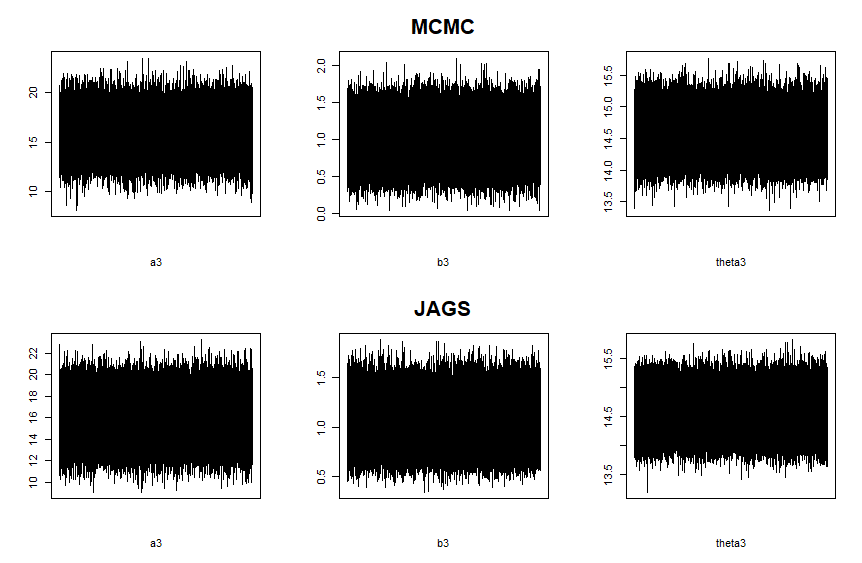
\includegraphics[scale=0.5]{figs/trace.png}
    \caption{Trace plots for Zack Wheeler ($a_3, b_3, \theta_3$) under each sampling method. The trace plots for the other 5 pitchers are comparable.}
    \label{fig:trace}
\end{figure}

In addition to this random walk algorithm, I implemented the posterior sampling in \texttt{JAGS} to compare results. Trace plots from each sampling method are given in Figure \ref{fig:trace}, and additional convergence diagnostics are in Table \ref{tab:conv}. Recall that the acceptance rate is not applicable under JAGS, nor is it applicable for $\boldsymbol{\theta}$ in my MCMC because they were drawn from their full conditionals. Overall, I do think convergence and computational efficiency were better in JAGS, but there is no evidence to suggest serious issues with convergence using either method. In the next section, we will see that the results are extremely similar between both methods. The remainder of the analysis after that, however, proceeds with the samples obtained in JAGS.

\begin{table}[]
    \centering
    \begin{tabular}{lllllll}
    \toprule[1.5pt]
         & Parameters & Chains & Acceptance & ESS & Geweke & $\hat{R}$ \\
         \midrule
        MCMC & $\boldsymbol{a}$ & 1 & 0.55 & 32070 & .26 & NA \\
        & $\boldsymbol{b}$ & 1 & 0.28 & 50022 & .09 & NA \\
        & $\boldsymbol{\theta}$ & 1 & NA & 99673 & .09 & NA \\
        JAGS & $\boldsymbol{a}$ & 8 & NA & 158585 & .10 & 1 \\
        & $\boldsymbol{b}$ & 8 & NA & 158989 & 0.37 & 1 \\
        & $\boldsymbol{\theta}$ & 8 & NA & 159534 & .09 & 1 \\
        \bottomrule[1.5pt]
    \end{tabular}
    \caption{Convergence comparison between MCMC and JAGS.  1 chain was run for my MCMC, while 8 chains were run in JAGS (in parallel), leading to more overall iterations. Thus, $\hat{R}$ applied only to the chains from JAGS. The ESS column represents the mean effective sample size for all 6 parameters in that row. The Geweke column represents the minimum p-value for all 6 parameters in that row. None of these p-values were less than 0.05, so there is no indication that the end of the chains converged to a distribution different than the start of the chains.}
    \label{tab:conv}
\end{table}

\subsection{Posterior Summarization}

Pitch count data is sometimes very slightly right skewed (there may be a few innings where batters get on base more and force a higher pitch count). Thus, I believe that using absolute error loss and the posterior median of the samples is most appropriate for posterior point estimation on $\boldsymbol{\theta}$. Using the posterior mean could be more influenced by outlying data points. However, when we examine the posterior predictive distribution of $y^*$ later on, the mean will be used because the median would be much less informative when working with a discrete variable.

For each pitcher, the posterior median was computed as well as a 95\% credible interval and a 95\% Monte Carlo confidence interval. Because the sample size was so high, the Monte Carlo error was almost nonexistent and the confidence intervals are very close to the point estimate. Table \ref{tab:bayes-ests} displays these results both for the by-hand MCMC algorithm and the JAGS output, restricted to $\boldsymbol{\theta}$ for brevity. 

\begin{table}[h]
    \centering
    {\small %
    \begin{tabular}{llccc}
         \hline
         \textbf{MCMC} & Pitcher & Posterior Median & 95\% Credible Interval & 95\% MC Interval \\
         \hline
         $\theta_1$ & Walker Buehler & 14.718 & (14.16, 15.29) & (14.71977, 14.71978) \\
         $\theta_2$ & Nathan Eovaldi & 15.543 & (14.94, 16.17) & (15.54786, 15.54787) \\
         $\theta_3$ & Zack Wheeler & 14.585 & (14.05, 15.13) & (14.58555, 14.58556) \\
         $\theta_4$ & Taijuan Walker & 14.682 & (14.05, 15.33) & (14.68592, 14.68593) \\
         $\theta_5$ & Shane McClanahan & 15.663 & (14.90, 16.44) & (15.66531, 15.66532) \\
         $\theta_6$ & Max Fried & 15.130 & (14.49, 15.78) & (15.13280, 15.13281) \\
         \hline
         \textbf{JAGS} & Pitcher & Posterior Median & 95\% Credible Interval & 95\% MC Interval \\
         \hline
         $\theta_1$ & Walker Buehler & 14.713 & (14.16, 15.29) & (14.71576, 14.71576) \\
         $\theta_2$ & Nathan Eovaldi &  15.543 & (14.94, 16.16) & (15.54521, 15.54522) \\
         $\theta_3$ & Zack Wheeler & 14.580 & (14.05, 15.13) & (14.58233, 14.58234) \\
         $\theta_4$ & Taijuan Walker & 14.677 & (14.04, 15.33) & (14.68056, 14.68057) \\
         $\theta_5$ & Shane McClanahan & 15.660 & (14.91, 16.44) & (15.66372, 15.66373) \\
         $\theta_6$ & Max Fried & 15.128 & (14.50, 15.78) & (15.13112, 15.13112) \\
         \hline
    \end{tabular}
    }%   
    \caption{Posterior summarization under each method. The medians and credible intervals are virtually identical.}
    \label{tab:bayes-ests}
\end{table}

The remaining estimates for $\mathbf{a}$ and $\mathbf{b}$ are part of the code supplement. To visualize the difference between JAGS and the random walk, I took Walker Buehler as a case study and plotted the posterior densities of $a_1,b_1,\theta_1$ for each sampling method. As evidenced by Figure \ref{fig:buehler} and Table \ref{tab:bayes-ests}, the posterior distribution of $\theta_1$ and $a_1$ is nearly identical between the two methods. For $b_1$, JAGS generates a slightly tighter distribution with lower variance and a narrower credible interval; however, the posterior medians are still very close.

\begin{figure}[h]
    \centering
    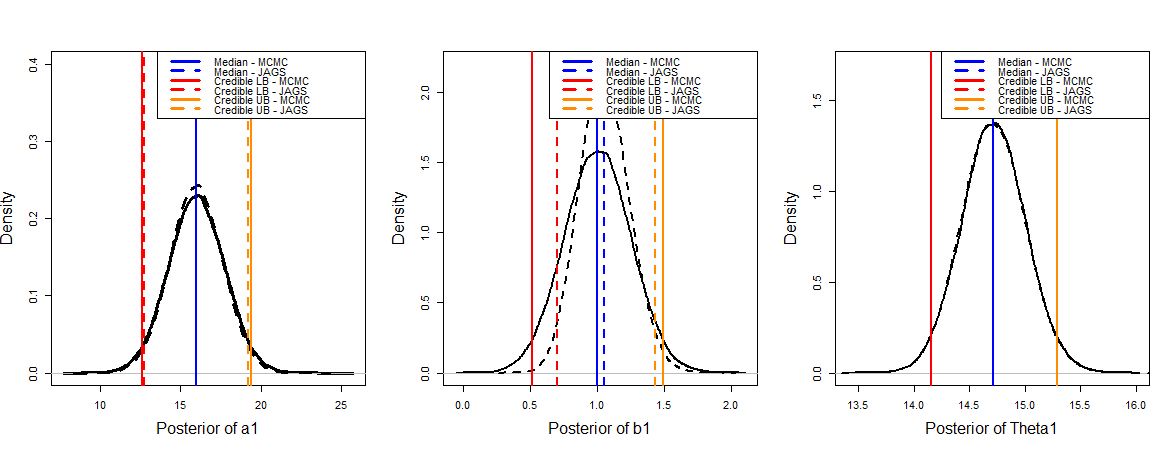
\includegraphics[scale=0.45]{figs/comp.png}
    \caption{Posterior densities of $a_1$, $b_1$, and $\theta_1$ which corresponds to Walker Buehler. Monte Carlo error bounds are not plotted because they are visually no different from the point estimates.}
    \label{fig:buehler}
\end{figure}

JAGS held many advantages over the random walk in terms of computational efficiency; it is easily parallelized and was able to run 8 chains in 11 seconds, while the random walk (which I did not parallelize, but could be with some extra implementation) ran 1 long chain in 11 minutes. JAGS returned samples with much weaker autocorrelation and an effective sample size nearly equivalent to the thinned number of iterations; the samples for $\mathbf{a}$ and $\mathbf{b}$ from the random walk had some autocorrelation even after thinning, and therefore has effective sample sizes of around 50 thousand. However, even though JAGS dominates the random walk both in computational and implementation time, the random walk is more flexible in design and allows us to experiment with various proposal distributions. The most important conclusion here is that the posterior sampling from the random walk and from JAGS are in general agreement with one another. I used the samples from JAGS to visualize the posterior distribution for each pitcher, that is, $\text{P}(\theta_j | \mathbf{y_j},a_j,b_j)$ in Figure \ref{fig:post}.

\begin{figure}[h]
    \centering
    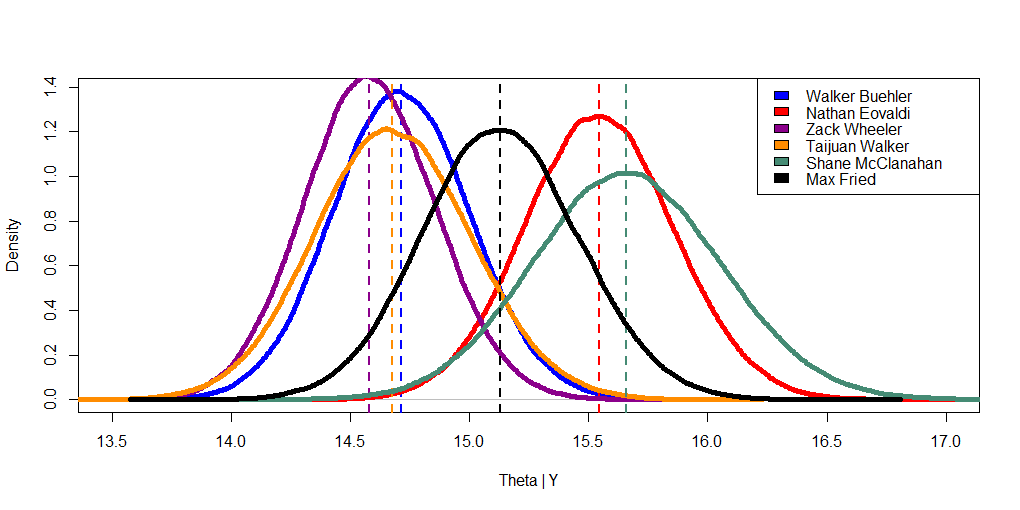
\includegraphics[scale=0.4]{figs/posterior.png}
    \caption{Posterior densities and point estimates of $\theta_j$ for each pitcher of interest. Zack Wheeler's curve falls lower than all others, agreeing with the exploratory findings from the introduction.}
    \label{fig:post}
\end{figure}

\subsection{Sensitivity Analysis}

Although the prior distributions for each $\theta_i, a_i, \text{and } b_i$ were not chosen arbitrarily, it is useful to examine the sensitivity of the model to varying prior distributions. There are two places where the prior distribution could be modified: in level 3, on the priors for $\mathbf{a}$ and $\mathbf{b}$, or in level 2, on the distribution of $\boldsymbol{\theta} | \mathbf{a}, \mathbf{b}$. In this section, I test the effect of three alternative priors (see Equation \ref{eq:alt-priors}) on the posterior distribution of $\boldsymbol{\theta}$.

\begin{align}
    \begin{split}
        \theta_i &\sim \text{Gamma}(a_i, b_i); \hspace{4pt} a_i \sim \text{N}(16, 1); \hspace{4pt} b_i \sim \text{N}(1,0.01) \\
        \theta_i &\sim \text{Gamma}(a_i, b_i); \hspace{4pt} a_i \sim \text{N}(32, 3); \hspace{4pt} b_i \sim \text{N}(2,\frac{1}{16}) \\
        \theta_i &\sim \text{N}(a_i, b_i); \hspace{4pt} a_i \sim \text{Unif}(14,17); \hspace{4pt} b_i \sim \text{Unif}(0.1, 1)
    \end{split}
    \label{eq:alt-priors}
\end{align}

Basically, the first alternative prior tightens the variances of $\mathbf{a}$ and $\mathbf{b}$, the second increases the means of $\mathbf{a}$ and $\mathbf{b}$, and the third modifies both levels of distributions entirely. Since the posterior summaries were virtually identical regardless of whether JAGS or my MCMC algorithm was used, I implemented the posterior sampling of these alternative models in JAGS only. As a case study, we examine the posterior distribution of $\theta_2$ (Nathan Eovaldi) to assess sensitivity. Figure \ref{fig:sens} shows the density of the four different prior distributions for $\theta_2$ (the one from our original model and then the three alternatives). Recall that because of the hierarchical structure, the prior density of $\theta_2$ is $\text{P}(\theta_2) \propto \text{P}(\theta_2|a_2,b_2) \text{P}(a_2)\text{P}(b_2)$. Evidently, the posterior distribution of $\theta_2$ is hardly affected by a change in the prior distributions.

\begin{figure}[h]
    \centering
    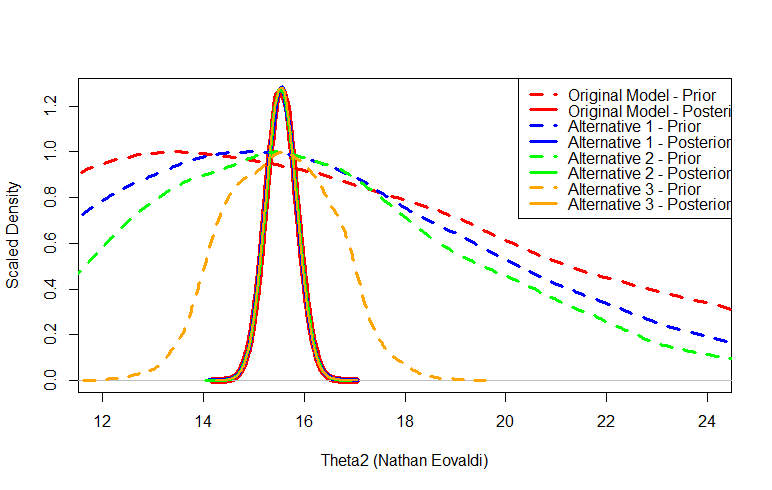
\includegraphics[scale=0.45]{figs/sensitivity.png}
    \caption{Four different prior distributions on $\theta_2$ and their resulting posteriors. The plots looks similar for the other 5 pitchers.}
    \label{fig:sens}
\end{figure}

To further verify the efficacy of the posterior distributions, I performed several posterior predictive checks on the model with replicated data using the test quantity $T(\boldsymbol{y}) = \frac{1}{n} \sum_{i=1}^{n_i} (\boldsymbol{y_j} - \theta_j)^2$, or the mean-squared error of the $j$th pitcher. There were no p-values below 0.11, so the tests did not raise any red flags and the details of these tests are included in the code supplement.

\subsection{Comparison to Non-Bayesian Methods}

Setting aside the first two levels of the hierarchical structure, a comparable non-Bayesian approach can be taken using the Poisson likelihood from the sampling model. A maximum likelihood estimator for any set of Poisson-distributed data is given by the sample mean, demonstrated in Equation \ref{eq:pois}. (Taking the second derivative would show that $\bar{y}$ is indeed a maximum, but is not included here for brevity).

\begin{align}
    \begin{split}
        L(\theta) &= \prod_{i=1}^n \frac{\theta^{y_i} e^{-\theta}}{y_i!} = \frac{\theta^{\sum y_i} e^{-n\theta}}{\prod_{i=1}^n y_i!} \\
        \ell(\theta) &= \sum y_i \log(\theta) - n\theta - \log(\prod_{i=1}^n y_i!) \\
        \ell^\prime(\theta) &= \frac{\sum y_i}{\theta} - n 
        \Longrightarrow \hat{\theta} = \frac{1}{n}\sum y_i = \bar{y}
        \label{eq:pois}
    \end{split}
\end{align}

Furthermore, Casella and Berger (2001) used the sufficient statistic $W=\sum y_i$ to obtain the formula for a $(1-\alpha)$\% confidence interval on $\theta$, which is given in Equation \ref{eq:ci}.

\begin{equation}
    \Big\{ \theta: \; \frac{1}{2n}\chi^2_{W,1-\alpha/2} \leq \theta \leq 
    \frac{1}{2n} \chi^2_{2(W+1),\alpha/2} \Big\}
    \label{eq:ci}
\end{equation}

From (\ref{eq:pois}) and (\ref{eq:ci}), we can obtain a point estimate of each pitcher's mean P/IP ($\theta_j$) and a corresponding 95\% confidence interval. These estimates and confidence intervals are given in Table \ref{tab:freq}, which can be compared to the Bayesian posterior medians and 95\% credible intervals from Table \ref{tab:bayes-ests}. Clearly, the results are very similar; however, as demonstrated in the next section, the Bayesian hierarchical model offers additional practical advantages in application.

\begin{table}[h]
    \centering
    \begin{tabular}{lccc}
         \hline
         Pitcher & Parameter & Sample Mean & 95\% Confidence Interval \\
         \hline
         Walker Buehler & $\theta_1$ & 14.713 & (14.16, 15.29) \\
         Nathan Eovaldi & $\theta_2$ &  15.544 & (14.94, 16.17) \\
         Zack Wheeler & $\theta_3$ & 14.579 & (14.04, 15.13) \\
         Taijuan Walker & $\theta_4$ & 14.676 & (14.04, 15.33) \\
         Shane McClanahan & $\theta_5$ & 15.663 & (14.90, 16.45) \\
         Max Fried & $\theta_6$ & 15.128 & (14.49, 15.78) \\
         \hline
    \end{tabular}
    \caption{Point and interval estimates for $\theta_1, \hdots, \theta_6$ using maximum likelihood and the Poisson 95\% confidence interval.}
    \label{tab:freq}
\end{table}


\section{Predictive Applications}

The individuals to whom this analysis is most applicable are the managers and front offices of the 30 Major League Baseball teams, especially those with starting pitchers on their staff who have recently returned from Tommy John surgery. The hierarchical model proposed can be used to predict the pitches thrown in a new inning for one of the six pitchers of study, or it can be used to generate a predictive distribution for a new pitcher of interest entirely. In this section I outline both of these procedures, and then offer insight as to how the posterior distributions of $\mathbf{a}$ and $\mathbf{b}$ can be used in additional studies. 

\subsection{Prediction of Future Start for Current Pitcher}

For each of the six pitchers studies in the analysis, I sampled 160000 sets of new predictive observations $y^*_1, \hdots, y^*_6$ using the 160000 samples of $\mathbf{\theta}$ from JAGS. The predictive distribution for each pitcher (Figure \ref{fig:preds}) has much higher variance than the posterior distribution of $\theta_i$, and is restricted to discrete draws because it comes from the Poisson likelihood instead of a conditional gamma distribution. The predictive distribution could be used to predict the probability of throwing above or below a certain number of pitches in the coming inning, allowing the manager to have more certainty in maintaining a limiting pitch count for his starter. For example, if the manager of the Tampa Bay Rays has Shane McClanahan at 90 pitches after 5 innings, and is trying to decide whether to send him out for the sixth, the predictive distribution could be used to estimate the probability of McClanahan completing the inning in 10 pitches or less. In his case, that probability is estimated at 9.05\%, but for Zack Wheeler, that probability is 14.18\%.

\begin{figure}[h]
    \centering
    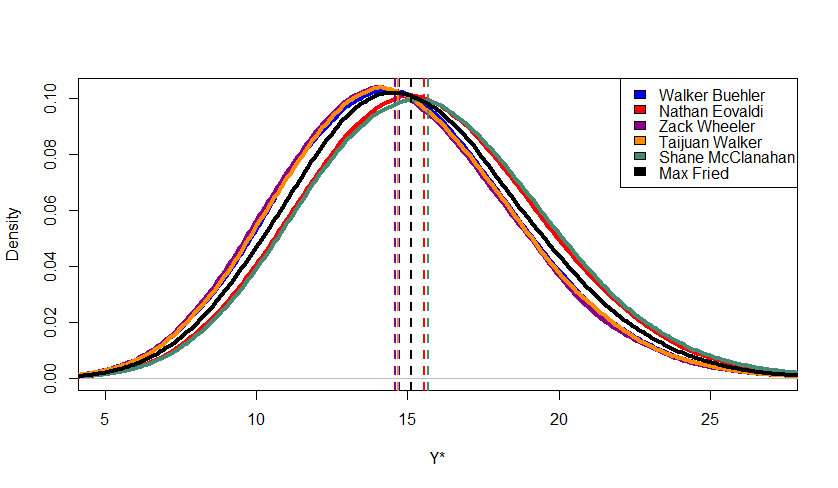
\includegraphics[scale=0.38]{figs/preds.png}
    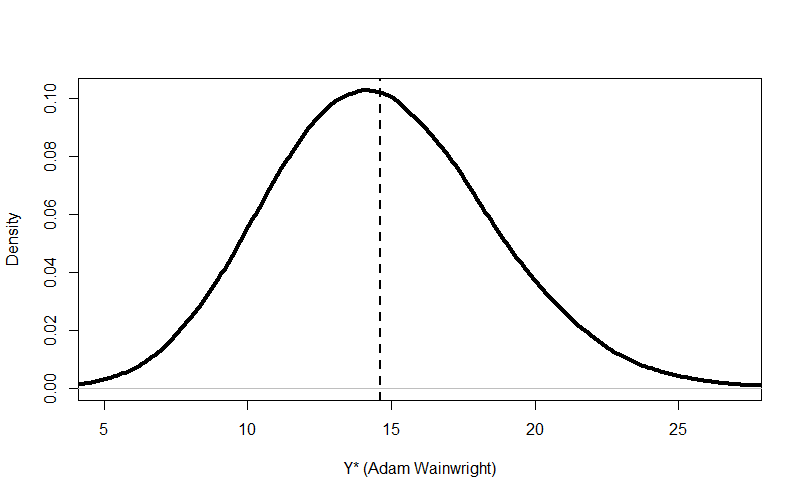
\includegraphics[scale=0.37]{figs/ww.png}
    \caption{(Left) Posterior predictive density for each pitcher. The dotted lines now represent the means rather than the medians, since the median would be exactly 15 for most of the pitchers and would not convey much information visually. (Right) The predictive density for Adam Wainwright of the St. Louis Cardinals, another Tommy John comeback pitcher. His average projected P/IP falls in between that of Zack Wheeler and Taijuan Walker. }
    \label{fig:preds}
\end{figure}


\subsection{Prediction for New Pitchers}

In addition, we could collect pitch data from the 2021 season for a new starting pitcher and use the same model to predict their P/IP. It is possible to also estimate the parameters $\theta, a, b$ in the process, but if prediction is the only pertinent goal, we can re-run the model to get just the predictive samples. The other half of Figure \ref{fig:preds} shows this predictive density for Adam Wainwright of the St. Louis Cardinals, another pitcher who returned from Tommy John surgery several years ago.

\subsection{Posterior Summaries of the Hyperparameters}

For the majority of this analysis, the entire focus has been on the parameters $\theta_1, \hdots, \theta_6$ rather than the estimates for $\mathbf{a}$ and $\mathbf{b}$. It is true that for direct application and prediction, the estimates for $\boldsymbol{\theta}$ are more important than those of $\mathbf{a}$ and $\mathbf{b}$. However, consider how the estimates of $\mathbf{a}$ and $\mathbf{b}$ could be used in further transformation-based analysis. For example, suppose MLB lowers the height of the pitching mound (which is an idea they have entertained, due to the decrease in batting average over the last 20 years). With some preliminary data of how much pitch count has increased overall due to the change, we could  modify the scale parameter (or the inverse rate, in our case) accordingly with almost no computational effort. 

Estimating $\mathbf{a}$ and $\mathbf{b}$ is also just generally helpful in understanding the nature of the distribution for each $\theta_j$. For instance, the posterior median of $a_5$ is higher than all other $a_j$, and the posterior median of $b_5$ is lower than all other $b_j$, leading to the conclusion that the variance of the mean for Shane McClanahan's pitch count is more spread out. In other words, we have a little more uncertainty in estimating $\theta_5$ for McClanahan.


\section{Conclusion}

The goal of the study was to use a statistical model to summarize pitch counts for pitchers who have returned from Tommy John surgery in recent years. I proposed a Bayesian hierarchical model structure and implemented it for six different pitchers: Buehler, Eovaldi, Wheeler, Walker, McClanahan, and Fried. The study detailed two different methods to sample from the posterior distribution of this model and estimate $\theta_j$, or the mean number of P/IP for pitcher $j$, and allowed us to compare the pitch efficiency between pitchers. These methods (the random walk and JAGS) produced output consistent with one another, up to Monte Carlo error. A sensitivity analysis showed these posterior distributions were robust to the choice of priors. For further verification, point and interval estimates were computed from the frequentist paradigm and compared to the Bayesian estimates.

Obviously, every pitcher is different due to a variety of factors - their age, the team they play for, the team they are facing, and their health history, among others. I accounted for this in the hierarchical model by assigning unique, non-exchangebale parameters $\theta_j, a_j, b_j$ to each pitcher; however, this does not take into account the actual characteristics of each game started. For future analysis, a Bayesian regression model could be implemented to replace the first level of our hierarchical model and incorporate a set of covariates in sampling $\theta_j, a_j, \text{and } b_j$.

The central contribution of the study is that samples can be obtained from a posterior predictive distribution for any given pitcher, which establishes a direct application to baseball teams trying to determine the longevity of their starters in any given game.


\end{document}
